%----------------------------------------------------------------------------------------
%	PACKAGES AND OTHER DOCUMENT CONFIGURATIONS
%----------------------------------------------------------------------------------------


\documentclass[12pt,oneside,final,a4paper]{report}
\usepackage{generators/imports}
\usepackage{listings}
%\makeglossaries      % alt 1
\makenoidxglossaries  % alt 2

\renewcommand*{\acronymname}{List of Acronyms and Abbreviations}
\renewcommand{\glsnamefont}[1]{\textbf{#1}}

%Create acronyms here.
%\newacronym{nn}{NN}{Neural Network}
\newacronym{gnn}{GNN}{Graph Neural Network}
\newacronym{vcs}{VCS}{Version Control System}
%\newacronym{ml}{ML}{Machine Learning}
%\newacronym{ai}{AI}{Artificial Intelligence}
\newacronym{co}{CO}{Combinatorial Optimization}
\newacronym{mwm}{MWM}{Maximum Weighted Matching}
\newacronym{mis}{MIS}{Maximal Indepndent Set}


%You can also do explanations.
\newglossaryentry{git}{name={Git},
    description={Git and GitHub is a \gls{vcs} for tracking changes in computer files and coordinating work on those files among multiple people}}
\newglossaryentry{ga}{name={Greedy Algorithm},
    description={Algorithm that usually tries to sort input based on some criteria and then naively produces the answer based on the order of sorting}}
\newglossaryentry{ai}{name={Artificial Intelligence},
    description={Artificial Intelligence is a field of study regarding intelligence simulated by computers. Where intelligence is meant in context of human intelligence}}
\newglossaryentry{ml}{name={Machine Learning},
    description={Machine Learning studies algorithms that learn general patterns and make predictions based on some form of input. It is one form of \gls{ai}}}
\newglossaryentry{nn}{name={Neural Network},
    description={Neural Network is one of many technologies used in\gls{ml}}}


\begin{document}
\begin{titlepage}

\newcommand{\HRule}{\rule{\linewidth}{0.5mm}} % Defines a new command for the horizontal lines, change thickness here

\center % Center everything on the page
 
%----------------------------------------------------------------------------------------
%	HEADING SECTIONS
%----------------------------------------------------------------------------------------

\textsc{\LARGE University of Bergen \\ Department of Informatics}\\[1.5cm] % Name of your university/college

%----------------------------------------------------------------------------------------
%	TITLE SECTION
%----------------------------------------------------------------------------------------

\HRule \\[0.5cm]
\begin{Huge}
	\bfseries{Solving Maximum Weighted Matching problem using Graph Neural Networks}\\[0.7cm] % Title of your document
\end{Huge}
\HRule \\[0.5cm]

%----------------------------------------------------------------------------------------
%	AUTHOR SECTION
%----------------------------------------------------------------------------------------

\large \emph{Author:} Nikita Zaicev\\
\large \emph{Supervisor:} Fredrik Manne\\[2cm]

%----------------------------------------------------------------------------------------
%   LOGO SECTION
% 	This will require the graphicx package
%	Change the line to comment if you only want the UiB Logo
%	Logo for other faculties here: http://kapd.h.uib.no/profilmanual/99LastNed/99a_lastned.html
%----------------------------------------------------------------------------------------

\centerline{
\includegraphics[scale=1.9]{figures/canvasWithFaculty}}
%\centerline{
\includegraphics[scale=0.15]{figures/canvas}}  %change for your faculty

%----------------------------------------------------------------------------------------
%	DATE SECTION
%----------------------------------------------------------------------------------------

{\large \monthyeardate\today}\\[3cm] % Date, change the \today to a set date if you want to be precise

%----------------------------------------------------------------------------------------
%	LOGO SECTION
%----------------------------------------------------------------------------------------

\vfill % Fill the rest of the page with whitespace

\end{titlepage}
 % This is the titlepage
\pagenumbering{roman}

\begin{abstract} 

\noindent In this work we tried to train a \gls{gnn} to solve the Maximum Weighted Matching problem on graphs. 

\end{abstract}

\renewcommand{\abstractname}{Acknowledgements}
\begin{abstract}
	I want to thank Fredrikk Manne, Kenneth Langedal and Johannes Langguth for helping me with this work.
	
	\vspace{1cm}
	\hspace*{\fill}\texttt{Nikita Zaicev}\\ 
	\hspace*{\fill}\today
\end{abstract}
\setcounter{page}{1}
\newpage
{
\tableofcontents 
\let\cleardoublepage\clearpage \listoffigures 
\let\cleardoublepage\clearpage \listoftables 
\let\cleardoublepage\clearpage \lstlistoflistings
}
\pagenumbering{arabic}
\setcounter{page}{1}
\setlength{\parskip}{0.5cm plus4mm minus3mm}  

\include{chapter/Introduction}
\chapter{Background}
\label{sec:background}

This Chapter focuses on the history, applications and impact of machine learning and goes through core concepts and ideas behind neural networks and graph neural networks. Relevant information about \gls{co}, graphs, exact and approximation algorithms is also included here.

\section{Neural Networks and Machine Learning}

Machine learning in computer science is a broad term for all the models and algorithms that use statistical methods to learn patterns and make predictions. Some of the earliest algorithms were invented in the 1940s \cite{mlhist}, but the viability was limited by the lack of data and computational power. One of the first works that began using GPUs to speed up the training process were Raina et al.\ \cite{fistgpuuse} in 2009. Both GPU and machine learning technologies have been improving ever since. The use of neural networks has found a place in almost every field. 

Neural network is a statistical method in machine learning inspired by the way brains work. The areas in which this method is applied include classification tasks that aim to identify certain objects based on their features, such as Iris flower classification \cite{swain2012approach} presented by Swain et al. A family of Iris flowers can be split into three categories based on the features, such as the shapes of petals and sepals. Iris flower classification is a good and simple example of a classification problem where the input is the lengths and widths of petals and sepals, and the task of the neural network is to put every flower in the correct category based on these input features. Other complex problems such as image recognition of pathogens \cite{TRAORE2018257} have also been solved by using neural networks. Besides recognition and classification, neural networks have also found applications in the synthesis of data, such as text generation with ChatGPT \cite{RAY2023121} and image generation \cite{Liao2022CVPR}. From around 2017, the Graph Neural Network (GNN) subclass of neural networks started to gain more traction \cite{hamilton2018inductive}, \cite{velickovic2018graph}, \cite{kipf2017semisupervised}. The \gls{gnn}s are specialized for working with graph data as the name suggests and are the main topic of this work, but before describing the \gls{gnn}s in more detail, let us revisit the basics of machine learning and neural networks.

Machine learning can be split into supervised, unsupervised and reinforcement learning. 

In the case of supervised learning, the machine learning model is given training data with the correct answers. The model can then learn from this by trial and error and then apply gained knowledge to the unseen data. 

Supervised learning requires a dataset with precomputed answers. It is common to split the dataset into three parts: training, validation and test. Training is used to train the model, while validation is used to evaluate several models trained on the same training dataset, but with different parameters for models learning process. The test dataset is the final data set used to evaluate the final model, since the model was chosen based on the validation dataset and needs to be tested on unseen data to avoid bias. This approach relies on feeding the model large amounts of data in order to cover as much variety in data as possible. The training process can take days, but on the positive side, after the model is done with training, the running time of making a prediction can be as low as $O(n)$ in the case of simple neural networks, although it depends on the architecture. 

In the case of unsupervised learning, the model lacks the correct answers and has to use other means to calculate the error and adjust weights. Autoencoders are an example of such networks and rely on two separate neural networks, where one part attempts to encode data and the other to decode it and give feedback based on how close the decoded data is to the original. 

Reinforcement learning is less relevant, since it is used in cases with no training data. And in this work we have data in the form of graphs. Therefore, in this thesis, we are using supervised learning, where a neural network is trained on a dataset of graphs with optimal solutions found using an exact algorithm. 

Neural networks are a subclass of machine learning algorithms that are inspired by the human brain. They are, for the most part, made of different layers that consist of “neurons”. Layers can be grouped into three types: an input layer that reads the given data, one or more middle layers that process the data and an output layer that gives the final answer. In a simple neural network, each neuron in a layer is usually connected to all the neurons of the next layer, although it often depends on the architecture. 

\begin{figure}[H]
    \centering
    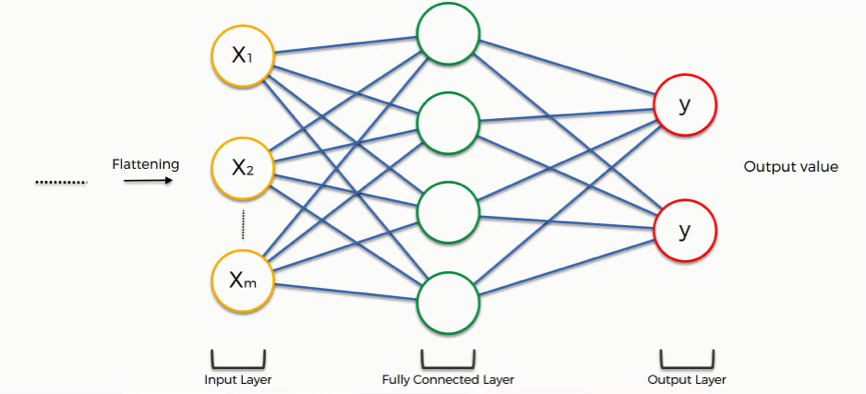
\includegraphics[scale=0.9]{figures/ffcexample}
    \captionsource{Simple neural network example}{https://www.superdatascience.com/blogs/convolutional-neural-networks-cnn-step-4-full-connection}
    \label{Simple neural network example}
\end{figure}

Figure \ref{Simple neural network example} visualizes how a simple fully connected neural network might look. The flattening refers to formatting the input features as a one-dimensional array to match the input layer size. This type of neural network is called fully connected, since each neuron is connected to every neuron in the next layer. The output layer represents the final binary classification step, where the two neurons stand for each of the two total categories this network is designed to identify.

Neuron connections have assigned weights. When the neural network model receives input, it is passed through the layers and gets multiplied by the weights. Assume an input neuron with value $x1$ is passed to a neuron in the next layer. The value of the neuron in the next layer will then be $w1(x1) + b1$, where $w1$ is the weight between the nodes and $b1$ is the bias term used to improve models flexibility. One might have noticed that the formula for passing data from one neurn to the other is a simple linear function. After the passing is done and the output layer is reached, the result in the output layer is some altered numerical representation of the input that can, depending on the goal, be interpreted as some prediction. For example, by applying a Softmax function on the output of the model, the result of each neuron would be between 0 and 1, and could be treated as the probabilities. This is a common way to do classification tasks. 

\begin{figure}[H]
    \centering
    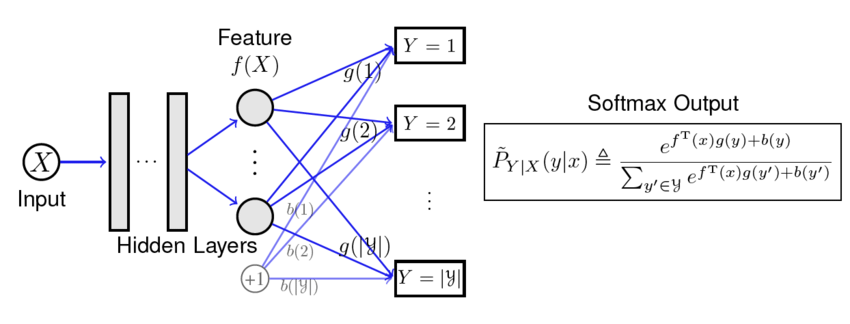
\includegraphics[scale=0.6]{figures/classificationExample}
    \caption{Classification example}
    \label{Classification example}
\end{figure}

Figure \ref{Classification example} shows another example of a classification network. This network has multiple hidden layers and an output layer with multiple classes from the set $Y$. To output the probabilities of an item being in each of the classes, the values from the output neurons are passed through the $softmax$ function.

Neurons also require an activation function to introduce non-linearity into the model. Without non-linearity, the multiplication of weights from each layer would result in a function that can be represented as a single linear transformation, defeating the purpose of having multiple layers in the architecture. A commonly used activation function is ReLU $max(0,x)$.

To teach the model, the weights of the neural network can be adjusted depending on the accuracy of the predictions by methods called back-propagation and gradient descend. Back-propagation calculates the impact of each weight on the total error using derivation. The error is calculated using a loss function such as negative log likelihood \[\text{NLL} = - \sum_{i=1}^{N} \sum_{j=1}^{C} y_{ij} \log(\hat{y}_{ij})\], where $N$ is the number of items, $C$ is the number of classes, $y_{ij}$ is $0$ or $1$ depending on whether class $j$ is correct for item $i$ and $\hat{y}_{ij}$ is the predicted class. Then, the gradient descend method is used to adjust the weights and potentialy lower the error in the next iteration. This process can be repeated multiple times, until the model can make predictions well enough. The process is fittingly called training. An important thing to keep in mind is that a trained model needs to be tested on unseen data since it can memorize all the data it was trained on. Overfitting is a term describing a model that learns the patterns of the training dataset near perfectly without being able to keep the same performance when given unseen data. In machine learning, one is interested in generalization, the model needs to find patterns that are common for all the relevant data it can encounter.

One epoch is described as one iteration of training where the model has gone through all the training data once. The number of epochs or how long the model must be trained depends heavily on the parameters and how complex the patterns are. Training can be stopped after a set number of epochs, if the information loss is nearing zero or when the loss plateaued indicating that the model cannot improve.

\section{Graphs}

The following gives a short introduction to what a graph is and the graph terminology used in this work.

A graph $G$ is a pair $(V,E)$, where $V$ is a set of vertices and $E$ is a set of edges between the vertices $E \subseteq \{(v,u) |  v,u \in V\}$ \cite{graphdef}. Two vertices with an edge between them are adjacent or connected. In an undirected graph an edge implies that the connection is bidirectional, meaning $(v,u)$ and $(u,v)$ are equivalent. Figure \ref{The difference between a directed and an undirected graph} demonstrates the difference between an undirected graph (right) and a directed graph (right).

\begin{figure}[H]
    \centering
    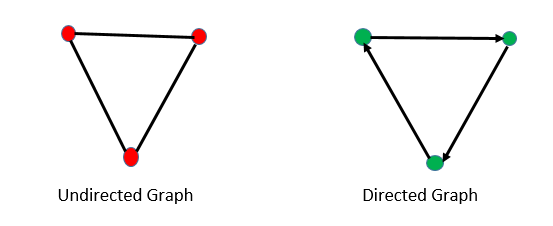
\includegraphics[scale=0.7]{figures/graph-theory}
    \captionsource{The difference between a directed and an undirected graph}{https://byjus.com/maths/graph-theory/}
    \label{The difference between a directed and an undirected graph}
\end{figure}

For graphs with weighted edges, let $W()$ be a weight function on the edges such that $W(e) \rightarrow \mathbb{Q}^+$ 

In this work we convert graphs to their line graph representation. The line graph is a complement of the original graph that turns each edge to a vertex and connects the vertices if they shared a vertex in the original graph. A simple example of a graph and its line graph can be seen in figure \ref{Line graph figure}.

\begin{figure}[H]
    \centering
    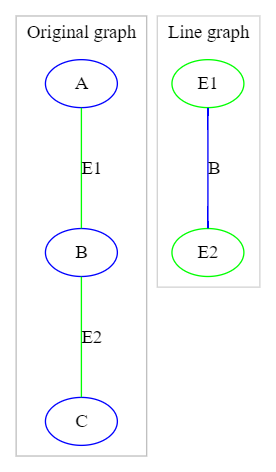
\includegraphics[scale=0.3]{figures/LineGraphExample}
    \caption{Original graph (left) and its line graph (right)}
    \label{Line graph figure}
\end{figure}

Note that the line graph willl always have the number of nodes equal to the number of edges in the original graph while, the number of edges in the line graph can vary and can be higher than the number of the original nodes.

In general, for graphs we use following notations: 
$$nodes/vertices: v \in V,$$
$$edges: e_{v,w} \in E | v, w \in V$$
$$neighbourhoods: N(v) \subseteq \{w, (v,w) \in E\}.$$ 

\section{Graph Neural Networks}
\label{sec:graphneuralnetworks}
Graph Neural Network (\gls{gnn}) is a relatively young subclass of neural networks designed specifically for solving graph related problems, and has been a growing topic of research in the last couple of years. \gls{gnn}s in general can be used for three purposes: graph prediction, node prediction and edge prediction. Graph prediction can be used to find graphs with desired properties, for example, to determine if a graph has cycles in it. Similarly, node and edge prediction is applicable to classification problems, such as identifying nodes and edges that are part of a cycle.

The application of graph prediction can be seen in bioinformatics. Ramachandran et al.\ have used graph convolutional network to predict how different proteins interact with each other \cite{ramachandran2019protein}. Node-level prediction has found application in traffic forecasting \cite{Yu2018}. Edge or link prediction models can be seen in the context of social networks with applications such as friends recommendation \cite{ADAMIC2003211}. Another popular field for \gls{gnn} research is Combinatorial Optimization (\gls{co}), which leads us to the well known problems such as the Maximum Weighted Matching (\gls{mwm}) and Maximal Independent Set (\gls{mis}).

Brusca et al.\ \cite{brusca2023maximum} showed a self-training \gls{gnn} for \gls{mis}. 

Schuetz et al.\ made an unsupervised \gls{gnn} \cite{Schuetz2022} for solving \gls{mis} and Angelini and Ricci-Tersenghi \cite{Angelini2022} compared its performance to greedy algorithms and reported some problems with \gls{gnn}s performance.

The reason \gls{mis} solving is mentioned is because the problem is to some degree related to \gls{mwm}, as algorithmic problems often are. There are concrete examples in the Methodology and Data chapter. \gls{mis} is also more often a subject for research, while research on \gls{mwm} is not that common. There are, however, some examples such as Wu and Li trying to solve \gls{mwm} using deep reinforcement learning \cite{WU2022400}. In this work they reported that their model outperforms state-of-the-art algorithms.

\gls{gnn}s are based on the same concepts as simple neural networks, but with some modifications to better suit graph, node and edge recognition problems. A simple \gls{gnn} can use a fully connected layer on each node and edge, as well as on the whole graph at once to generate a new numericatal representation for each element called embedding. In the following figure \ref{GNN example} one can see a simple overview of how the graph's information is passed from one layer to another, where $V$ denotes nodes, $E$ edges, $U$ graph-level features and update function is a neural network layer.

\begin{figure}[H]
    \centering
    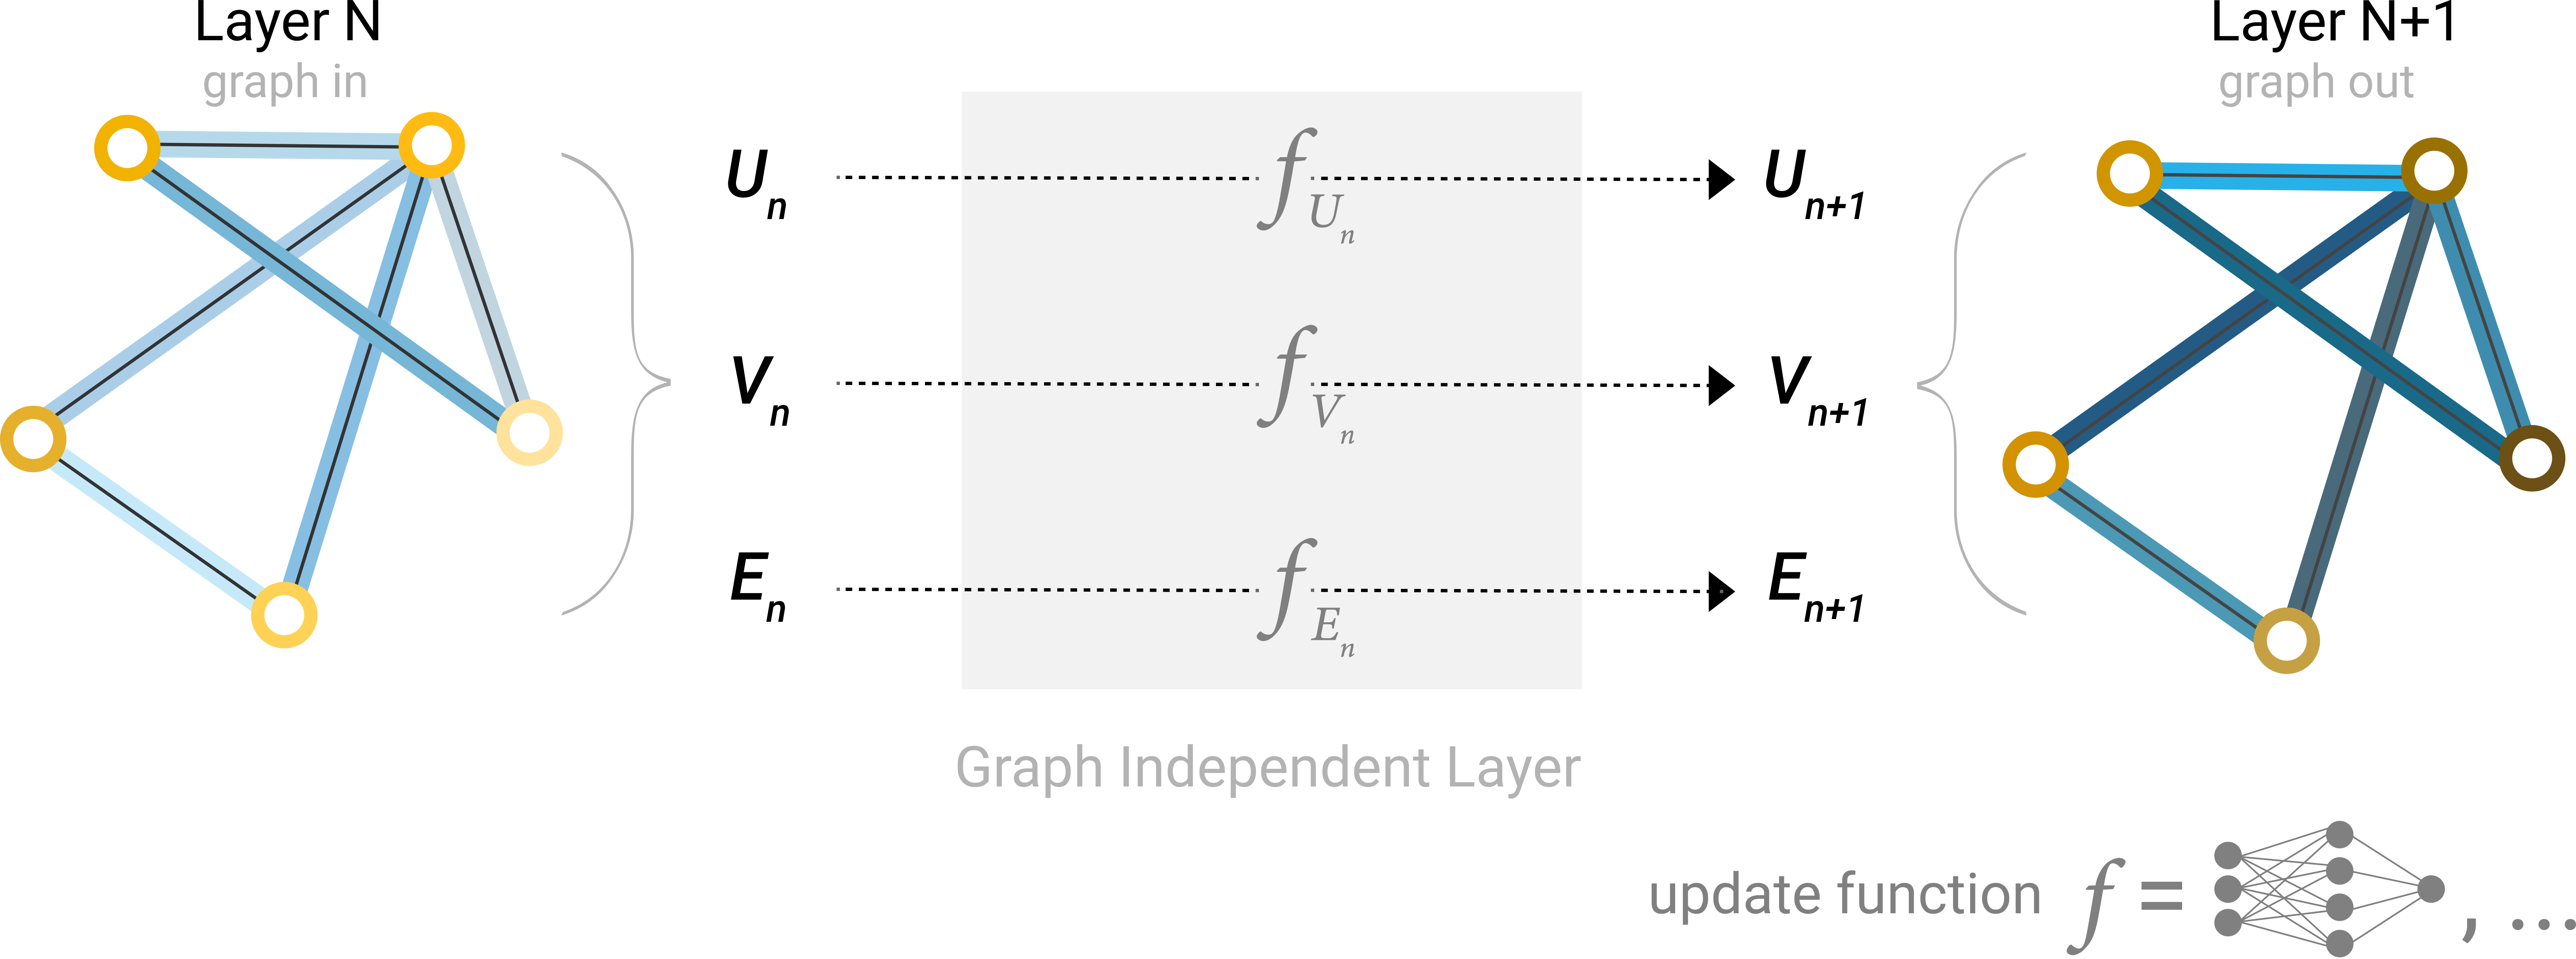
\includegraphics[scale=0.8]{figures/gnnintro}
    \captionsource{GNN example}{https://distill.pub/2021/gnn-intro/}
    \label{GNN example}
\end{figure}

For a simple node classification example, assume a graph with some nodes, where each node has two numerical features $f1$ and $f2$. Assume a \gls{gnn} that uses a simple fully connected network, where the input layer has two neurons, the middle layer has five and the output layer has two. For each node, the input layer reads the two features. Values of these features are then multiplied by the weights between each input neuron and each neuron in the next layer. One can express it as a matrix multiplication: 
$$
\begin{pmatrix}
f1 & f2 
\end{pmatrix}	
\times
\begin{pmatrix}
w11 & w12 & w13 & w14 & w15 \\
w21 & w22 & w23 & w24 & w25
\end{pmatrix}	
=
\begin{pmatrix}
n1 & n2 & n3 & n4 & n5 \\
\end{pmatrix}	
$$

Where the $f1, f2$ are node features and $w11$ to $w15$ are the five weights between the $f1$ input neuron and all the neurons in the next layers.

The information is then similarly passed from the middle layer to the output layer. The initial values of the node features have now been changed by the weights between the neurons, resulting in two output features. The \gls{gnn} has now produced an embedding for each node. Yet, the embeddings by themselves are not enough. In this example, the \gls{gnn} does not utilize the structure of the graph and the embedding of each node is not affected by its neighbours. 

If one wants to classify the nodes based on the node features only, then it can be done by using a standard neural network. However, for graphs, one is interested not only in the isolated node features, but in the nodes' relation to their neighbours. Additionally, graphs are not guaranteed to have any features for nodes and edges. 

What if one wants to use edges for classification of the nodes? In that case \gls{gnn} can use a pooling method. Pooling uses an aggregation function such as summation to sum together all the edge embeddings that a node has, and produce a new embedding. Alternatively, one can use neighbouring nodes for the same purpose, which leads to the specific type of \gls{gnn}s.

\gls{gcn} is one of the subclasses of \gls{gnn}s with some resemblance to the \gls{cnn}s used in image recognition. \gls{gcn} uses message passing to make use of the graphs' structure. For nodes, message passing gathers neighbouring node embeddings, aggregates the embeddings and then passes them through the network. The following figure \ref{Message passing example} shows how features from the neighbouring nodes are aggregated and passed to the next layer.

\begin{figure}[H]   
    \centering
    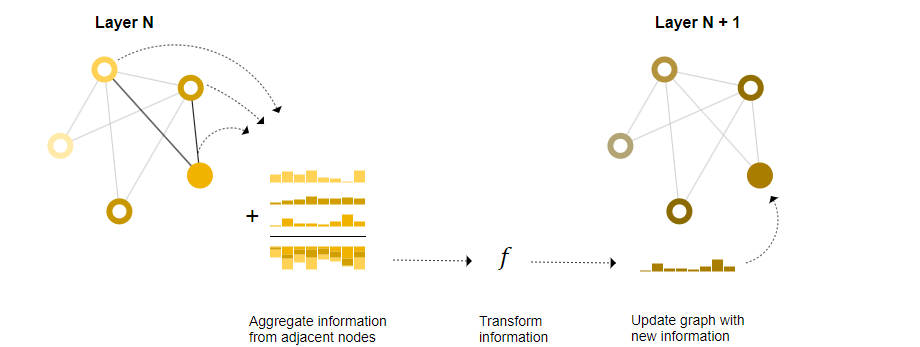
\includegraphics[scale=0.7]{figures/messagepassing}
    \captionsource{Message passing example}{https://distill.pub/2021/gnn-intro/}
    \label{Message passing example}
\end{figure}

Adding more layers increases the depth of the neighbourhood used. Meaning if a model has two layers, when passing through the second layer the embeddings of the neighbours are already an aggregation of its neighbours. This allows the \gls{gnn}s to utilize graph structure in a way that other neural networks cannot.

\begin{figure}[H]
    \centering
    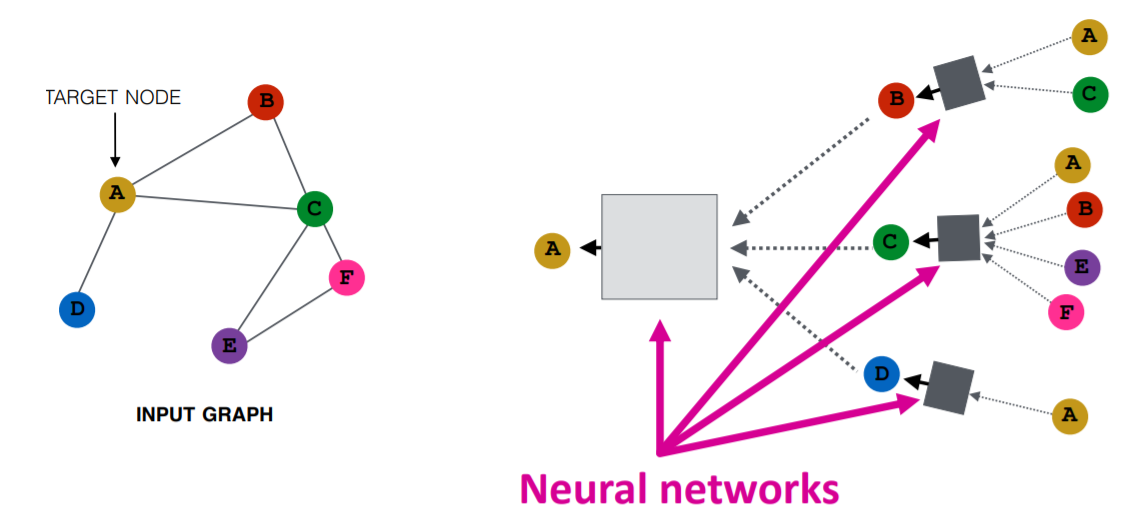
\includegraphics[scale=0.4]{figures/GNNExample}
    \captionsource{GCN example}{https://www.datacamp.com/tutorial/comprehensive-introduction-graph-neural-networks-gnns-tutorial}
    \label{GCN example}
\end{figure}

Figure \ref{GCN example} shows how two graph convolution layers affect a single node A.

\section{Implementation, training and hyperparameters}
\label{sec:implementation}

We have now gone through how \gls{gnn}s work from a high level view. However, it remains to create a \gls{gnn} as well as to train it. In this work we use \gls{pyg} library \cite{pytorchlib} that provides both the impementation for the various \gls{gnn} architectures and the tools to train the models. 

\subsection{Implementation}

The code snippet below \ref{Creating GCN with Pytorch} demonstrates how to create a simple \gls{gcn} by inheriting the base class $torch.nn.Module$. 

\begin{lstlisting}[caption={Creating GCN with Pytorch}, label={Creating GCN with Pytorch}, language=Python]
import torch
import torch.nn.functional as F
from torch_geometric.nn import GCNConv, Linear

class MyGCN(torch.nn.Module):
    def __init__(self):
        super().__init__()
        self.conv1 = GCNConv(1, 64) # 1 feature per each node
        self.conv2 = GCNConv(64, 64)
        self.lin = Linear(64, 2) # 2 classes 

    def forward(self, graph):        
        x, edge_index, edge_weight = graph.x, graph.edge_index, graph.edge_weight
        
        x = self.conv1(x, edge_index, edge_weight)
        x = F.relu(x)
        
        x = self.conv2(x, edge_index, edge_weight)
        x = F.relu(x)
        
        x = self.lin(x)
        return F.log_softmax(x, dim=1)    
\end{lstlisting}

A module in Pytorch can be a part of a larger network or a whole network in this case. One can add layers to the network by assigning other modules within the initializer function. Here, we add three layers. The first layer, $self.conv1 = GCNConv(1,64)$ is the input layer with one input neuron and 64 output neurons. This layer will require all nodes to have exactly one feature. To connect the $conv1$ layer to the second one, $conv2$, they must have a matching number of output and input neurons (64 in this example) respectively. The output module $self.lin = Linear(64, 2)$, is a simple fully connected layer that maps output neurons from the $conv2$ to the two neurons representing the two possible predictions. For example, whether a node should or should not be in the solution. In the $forward$ function, one has to define the order in which the information will flow through the network. First, one has to read the input from the graph. The $x$ represents the array of node features. In this case, the array is of size one. The $edge\_index$ and $edge\_weight$ represent the edges and their weights respectively. The $torch.nn.functional$ library provides the tool for mathematical operations and is used to apply the $F.relu$ activation function to the neurons as well as $F.log\_softmax$ to the output. The $relu = max(0,x)$ activation function serves the purpose of adding non-linearity to the network, enabling it to form complex patterns. The $F.log\_softmax$ function maps the output values into the desired range for measuring the error. Which function is used depends on how the error is calculated.

\subsection{Training}

To train the model described above, the following procedure can be done, demonstrated in the next listing \ref{Training GCN with Pytorch}. 

\begin{lstlisting}[caption={Training GCN with Pytorch}, label={Training GCN with Pytorch}, language=Python]
import torch
import torch.nn.functional as F
from torch_geometric.loader import DataLoader

device = torch.device('cuda' if torch.cuda.is_available() else 'cpu')
loader = DataLoader(dataset, shuffle=True)
optimizer = torch.optim.Adam(list(model.parameters()), lr=0.0005)

for epoch in range(100):        
    for graph in loader:
        optimizer.zero_grad()
        
        graph = graph.to(device)
        out = model(graph).to(device)   
            
        loss = F.nll_loss(out, graph.y)
        loss.backward()

        optimizer.step()
\end{lstlisting}

First, the $DataLoader$ and optimizer are initialized. The $DataLoader$ is responsible for managing and preproccessing the data. In this case, it only shuffles the dataset items randomly. The optimizer is used to preform the gradient descent on the models weights. Adam \cite{ADAMIC2003211} is a commonly used optimizer that has several parameters such as learning rate (lr) that affect the training process and how the weights are updated. These parameters in the context of the model are called the model's hyperparameters. With dataloader and optimizer ready, the main training loop starts. For each epoch or iteration, we retrieve the next batch of data from the $dataloader$. Before updating weights, $optimizer.zero\_grad()$ is called to make sure that the optimizer's gradients are reset. Then we pass the graph to the GPU device if possible to speed up the calculations. The graph is then passed through the model with the output mapped using $log\_softmax$ within the model's forward function. The $log\_softmax$ mapping produces the logarithmic probabilities required by the $nll\_loss$ function to compute the error or information loss made from the model's output in regard to the correct answers contained in $graph.y$. The error is then propagated backward by calling $loss.backward()$, determining the impact each weight made and then $optimizer.step()$ updates the weights based on the current hyperparameters.

\subsection{Hyperparameters}

The term “hyperparameter” refers to the parameters used to adjust the training process and the architecture of the network, while “parameters” refer to the weights between neurons. In this work we test several hyperparameters that can be further split into categories.

The training and Adam optimizer related hyperparameters include:
\begin{itemize}
\item Epochs - the number of training iterations. The longer a model is trained the less errors it should make, given the sufficient complexity of the model.
\item Learning rate - by how much the weights of the model should be adjusted after each iteration. Small steps have a risk of a model getting stuck in a place where the changes do not improve the results, while a significantly different configuration of weights that gives better results might exist. Small steps also might require to train the model for longer to reach the desired level of performance. Too large learning rates have a risk of overstepping the better weight configurations.
\item Mini-Batching size - how many graphs are passed through the network before next weight adjustment. Passing data in batches can help to smooth the learning curve and reduce the risk of overfitting.
\item Class weights - how much should the model focus on a given class. Class weights can help with data imbalance where one class occurs more often than others. For example if 99\% of objects belong to one class, but the model needs to focus on finding the other 1\%. In our case the classes for the edges are: 
	\begin{itemize}
	\item 0 = is NOT in the solution.
	\item 1 = is in the solution.
	\end{itemize}	
\item Weight decay - used to keep \gls{gnn} weight values relatively small and decrease chances of the overfitting. 
\end{itemize}

The architecture related hyperparameters affect the capability of the network to learn complex patterns. 
\begin{itemize}
\item Network width - neurons in the layers.
\item Network depth - amount of layers. In case of \gls{gcn}s, the depth of the network also defines the radius of the aggregated node neighbourhood. 
\end{itemize}

The aggregation of neighbours is the key feature of the \gls{gnn}s and there are multiple functions that can be used.
\gls{gnn} specific hyperparameters:
\begin{itemize}
\item Aggregation function - the features of the neighbouring nodes can be aggregated by using different methods, including summation, maximum, minimum, multiplication and division.
\end{itemize}

Additionally one can experiment with adding extra features to the nodes during preprocessing or augmenting data. Examples of such features for the weighted graph are: 
\begin{itemize}
\item Degree - how many neighbours a node has
\item Sum of the weights. 
\end{itemize}
Such features can help the model to find new patterns.

The hyperparameter search helps to fit the model specifically for the desired task. In our case the model needs to learn how to solve Maximum Weighted Matching (MWM) on graphs.

\section{Maximum Weighted Matching and Combinatorial Optimization}

Combinatorial Optimization (CO) is a field of study that covers problems that require finding a subset or a combination of some set of elements that fulfills certain requirements. An example of such a problem would be Maximum Weighted Matching \gls{mwm} and Maximum Independent Set \gls{mis}. 

The \gls{mwm} problem asks to find a subset of edges in a weighted graph, such that the sum of weights is maximized, and each vertex appears only in one edge of that subset. More formally, given an undirected graph $G$ with a set of vertices $V$ and a set of weighted edges $E$, maximize total weight for set $S \subseteq E$, such that none of the edges in $S$ share vertices. In this work, the edges that are selected to be in the solution set will sometimes be referred to as “picked” and the ones that are not in the set “dropped”.

The \gls{mwm} problem is relatively simple compared to many others. It belongs to the field of \gls{co} and there are optimal algorithms for it that run in $O(|V|^{2}|E|)$ time, such as the blossom algorithm \cite{blossom}. Blossom algorithm is based on the blossom method for finding augmenting paths and the primal-dual method for finding a matching of maximum weight, both due to Jack Edmonds \cite{blossom}.

Optimal algorithms, however, can still be rather slow when working with large datasets, and in some cases an approximation algorithm may be more suitable as a solution if the exact answer is not critically important for the \gls{mwm} problem. The most simple example is a greedy algorithm that sorts all the edges by their weight and selects them in descending order. This is neither the only nor the best approximation algorithm, but rather a fast and simple one.

\begin{algorithm}
\caption{Greedy algorithm for Maximum Weighted Matching}\label{alg:cap}

\begin{algorithmic}
\State G(V,E)
\State $S = \emptyset$
\State $sortedE = descendingSort(E)$
\While{$sortedE \neq \emptyset$}
\State $e$ = first element in sortedE
\If{$e$ not adjacent to any edge in S}
  \State add e to $S$
  \State remove $e$ from sortedE
\EndIf
\EndWhile
\end{algorithmic}
\end{algorithm}

The running time of the Greedy algorithm is bound by the sorting, since the While loop iterates through the edges once and runs in $O(|E|)$. The fastest sorting runs in $O(|E| log(|E|))$.

To put \gls{mwm} in context, real world applications of matching algorithms can be found in scheduling problems such as transportation cost minimization \cite{mwmExample}, but are also often used as a part of larger algorithms.

Another problem that will be slightly touched is the Maximal Independent Set (\gls{mis}). \gls{mis} asks to find a subset of nodes such that no two nodes have an edge between them, and the total number of nodes is as large as possible. There is a similar problem \gls{mwis} which asks us to find an independent set in graph with weighted nodes that gives the largest total weight sum. \gls{mwis} is partially relevant as we use line graph transformation that essentially turns the original \gls{mwm} problem into \gls{mwis}.

\chapter{Research Methodology and Data}

This chapter focuses on describing which approaches were chosen for the task at hand and why, as well as shows how the work progressed. 

To reiterate the current problem is to find out if \gls{gnn} can compete at solving the \gls{mwm} problem compared to other approximation methods such as greedy algorithm.

\section{Challenges}

It is common to think of a neural network as of a black box where you give some data to this box and it tries to predict the correct answer. In this case the data is a graph consisting of vertices connected by edges that have weights and the expected answer should be pairs of vertices that were matched together.

As mentioned the idea behind supervised learning is to give a model the correct answers so it can by trial and error learn from it. Theese answers are not included in the initial datasets so the optimal solutions needs to be calculated. To find the optimal solution Blossom algorithm implemented by Joris van Rantwijk in Python was used \cite{mwmBlossom}. This does however point out an important weakness of the supervised approach. Obviously a model needs to be able to handle graphs of different sizes and it is the large ones that are most interesting. Finding an optimal for algorithmic problems for the large graphs can be time consuming, at the same time a model need as much data as possible to learn, leading to multiple large graphs consuming to much time combined. This poses a question whether it is possible for the model to learn on small and medium sized graphs that are not as time consuming and transfer learned patterns to solve larger graphs.

Another important aspect that must be taken in to the consideration is that it is unlikely for the model to fully follow the restictions of the problem. Model might decide to match same node to 2 neighbors at the same time, which should not be allowed. 

\section{Main Idea}

To summarize, given a weighted udirected graph, the \gls{nn} must predict  a valid subset of edges or in other words pairs of vertices that maximize the total weight. The \gls{nn} will have a graph as an input and the otput will be the probabilities (0.00 - 1.00) of how likely an edge will be in the matching. To control that a solution is valid, instead of picking all the edges with the probability higher than 50\%, the edges can be sorted by their probabilities and greedily picked in that order if they don't break the validity of the solution. This might sound illogical to use greedy algorithm on the models output to beat the normal greedy algorithm with weights, but the fact that edges are now sorted not by their weight, but a score decided by \gls{nn} does make a difference, since the \gls{gnn} can take multiple features in consideration when assigning probabilities. Some of these features come naturaly from the structure of the graph, and some we can manualy add during preprocessing. 

\gls{nn}s have a lot of hyperparameters and methods that can be tuned to make a model better suited for the task. The ideal way of finding the best combination of the hyperparameters is to try as many combinations as possible. Train a model for each combination and choose the one with best performance. This is a time consuming procedure however and therefore in this task the exploration of hyperparameters was narrowed down to the ones that seemed most important and indicated positive impact during early experiments. For training, Adam optimizer was used \cite{kingma2017adam}. Optimizer is used to adjust the weights of the network during training. Adam optimizer has several hyperparameters that can be usefull to achieve better results and is one of the popular optimizers to use.

During the experiments following hyperparameters were tested:
\begin{enumerate}
\item Learning rate - by how much the weights of the model should be corrected
\item Network depth - amount of layers 
\item Network width - neurons in the layers
\item Class weights - how much should the model focus on a given class. Classes being: 
	\begin{itemize}
	\item 0 = is NOT in the solution.
	\item 1 = is in the solution.
	\end{itemize}	
\item Weight decay - used to keep \gls{gnn} weight values relatively small and decrease chances of the model memorizing the answers. 

\item Additionally other methods were tried such as augmenting data (adding extra features to the nodes during preproccessing): 
	\begin{itemize}
	\item Degree - how many neighbours a node has
	\item Weight relative to the sum of neighbours.
	\item Weight difference from the sum of the neighbours.
	\item Sums of the weights. 
	\item 1st largest weight, 2nd largest weight.
	\end{itemize}

\end{enumerate}

\section{Data}

The model should be capable of solving any graph relevant to \gls{mwm} problem. A relevant graph can be difined by following characterisitcs
Ideally the model should be able to handle any kind of an udirected graph with weighted edges.

For training and experimenting with the \gls{gnn}, a MNIST dataset was used \cite{dwivedi2022benchmarking}. The dataset consists of 70000 relatively small graphs with 70 nodes and 564 edges on average. Graphs also include features for the edges representing distances between node. Theese features is what is used as the weights for the problem. Although the graphs in this dataset are relatively small they have some fitting qualities such and nodes having many neighbors creating more possible ways to match the nodes. Small size also makes it less time consuming to train the models and try different approaches as well as shows whether a \gls{gnn} trained on smaller graphs can transfer its knowledge to larger graphs.

Only training and testing on MNIST graphs does not represent all the different graphs that can occur, therefore model had to be tested on other graphs that have different structures and weight distributions. Model trained exclusively on MNIST dataset did not perform well on other graphs as one might ha expected. Therefore another dataset was made to cover larger variety of graphs. The dataset was a collection of random graphs from SuitSparse database that ranged between 100 and 10000 nodes. As described in more details in the \hyperref[sec:preprocessing]{Data preprocessing section}, some of the found graphs did not have edge weights. In these cases random weights were generated.

Including truly large graphs in training caused problems with insufficient memory and too long training time, but final model was still tested on some larger graphs than used in training. A couple large graphs from SuiteSparse were chosen for testing performance on large graphs with 40000 nodes and higher.

Small handcrafted graphs were used to test if \gls{gnn} can at least beat the cases specificaly made to abuse weaknesses of a greedy approach.

\section{Architecture}
\label{sec:architecture}
During the experiments the architecture of the \gls{gnn} model itself had mostly minor changes, but 2 rather different graph preproccessing steps were tried. In both cases we use \gls{gcn} layers (GCNConv) \cite{gcnpaper}. The GCNConv layer fits well for the purpose of this task because it makes use of the edge weights that are the crucial part for solving \gls{mwm}.

Python example:
\begin{lstlisting}[language=Python]
class MyGCN(torch.nn.Module):
    def __init__(self):
        super().__init__()
        self.conv1 = GCNConv(5, 640) # 5 features per each node, initialy 1
        self.conv2 = GCNConv(640, 640)
        self.lin = Linear(640, 2) # 2 classes 
\end{lstlisting}

Now, let us go through the whole process of a graph being matched using the \gls{gnn} presented here.

\subsection{Model pipeline}

As mentioned before one cannot fully trust the model to satisfy the restrictions of the problem. What is meant by the restrictions of the probem is the fact that every node can only be matched once. This is controlled by sorting the probabilities the model's outputs in descending order and adding matches to the final solution one by one, skipping matches that already have matched nodes. Another potential problem can happen at the end when some of the nodes that can be matched were not matched at all by the model. There is a chance of that happening, since only pick the matches with high enough probability are used. As a starting point probability threshold is 50\% and above. Two things are done to ensure nothing is left to waste. First, after the model is done the potential remainder of the graph is fed to the model again. For model this would essentialy just be a new graph and it may happen that model manages to match the remainder given the new context. This process can be repeated several times and the break condition is if 0 matches were made in the last iteration. At that point if anything is left, which hopefully is a small fraction of the initial graph, can be solved using standard greedy or any other approximation algorithm for that matter.

Passing the graph and it's consecutive remainders multiple times through the model can also be helpfull to deal with the case where one of the matches that was picked may play big role in how the rest of the solution will look like. Idealy to handle this case one might only pick one match at the time and pass the graph through the model again, but it will be too time consuming.

\subsection{Line Graph Approach}

Line graph approach was the first attempt at using a simple \gls{gnn}, which later turned out to be too time consuming for larger graphs to be worth further expriements. It did however give some usefull insight as well as a showed to be a proof of concept. In the context of graphs line graph is a complement of the original graph that turns each edge to a vertex and connects the vertices if they shared a vertex in the original graph. 

Examaple of a graph and its line graph convertion
\begin{figure}[H]
    \centering
    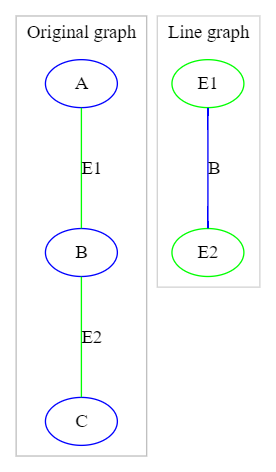
\includegraphics[scale=0.5]{figures/LineGraphExample}
    \caption{Original graph (left) and its line graph (right)}
    \label{Line graph figure}
\end{figure}

Converting to a line graph makes the architecture of the \gls{gnn} model simpler. Instead of needing to ask model for each pair of nodes is they should be matched together, the line graph model now can output the probability of a node being in the matching directly, since the node now represents two connected nodes from original graph. This also however transforms the problem itself. From the perspective og the model it is now trying to solve \gls{mwis}. \gls{gnn}s for \gls{mis} have been studied before. Nouranizadeh et. al. showed demonstrated a pooling method for solving \gls{mwis} \cite{DBLPjournals/corr/abs-2107-01410}. Unfortunately the large graphs can explode in size when converted to line graphs and were too time consuming in such cases.

\subsection{Edge Classification Approach}

A more natural way of approaching this problem is to give the model original graphs instead of transforming them to line graphs. But the model itselv only returns some numerical representation on the nodes in the graph. To get the predictions for the edges one can add a classifier module to the existing \gls{gnn}. This module's purpuse is to predict if a pair of two nodes will be in the matching. So the first part of the model produces embedding for each node and then for each edge, embeddings of both nodes are put together and passed to the classifier. Resulting in the model output being probabilities of all the edges being in the matching.

Python example:

\begin{lstlisting}[language=Python]

class MyGCNEdge(torch.nn.Module):
    def __init__(self):
        super().__init__()
        self.conv1 = GCNConv(7, 640)
        self.conv2 = GCNConv(640, 640)
        self.embed = Linear(1280, 80)

class EdgeClassifier(torch.nn.Module):
    def __init__(self):
        super().__init__()
        self.lin1 = Linear(160, 320) # 80 * 2 features since input is 2 nodes.
        self.lin2 = Linear(320, 2)

    def embedEdges(self, nodeEmbed, graph):
        x_src, x_dst = nodeEmbed[graph.edge_index[0]], nodeEmbed[graph.edge_index[1]]
        edgeEmbed = torch.cat([x_src, x_dst], dim=-1)        
        return edgeEmbed

\end{lstlisting}

\subsection{Data preprocessing}
\label{sec:preprocessing}
Not all graphs found in the database are fit for the training as is, and the ones that fit perfectly are few. Machine learning models require some preproccessing of data before it can be used. Convertion to the line graph is one example of such preproccessing. One might also need to augment the initial data to improve model performance. Finally machine learning models can be vulnerable to large numerical swings in the data, such as edge weights being higher than expected.

Most important are the edge weights. To ensure we have enough graphs to train on and the graphs cover a variety of structures, some of the chosen graphs that lacked weights recieved a randomly generated weights. The random weights had even distribution in the range between 0 and 1. All the graphs with preexisting weights were also adjusted to be in that range by shifting the weights to positive range if any negative weights were detected and then dividing by the largest weight. The weights could have been in any range, but the important thing is to have consistent weights for all the graphs. 

Another preprocessing step that was added is additional features for the nodes/vertices. This required different approaches for line graph and edge prediction approaches since in a line graph vertex represents an edge from the original graph. Line graph has weights assigned to the nodes themselves while using original graph nodes are assigned to edges.

One vertex feature does reamain in common: Degree of the nodes. Meaning how many neighbors each node has.

Line garphs node features:  

\begin{enumerate}
\item Weight relative to the sum of neighbours. For each vertex v:  \[ Wrel = v.weight  \div  (\sum_{n=0}^{|neighbors|} neighbors[n].weight) \]
\item Weight difference from the sum of the neighbours. For each vertex v:  \[ Wdiff = v.weight  \div  (\sum_{n=0}^{|neighbors|} neighbors[n].weight) \]
\item Sums of the neighbouring node weights. \[ (\sum_{n=0}^{|neighbors|} neighbors[n].weight) \]
\end{enumerate}

Normal graph edge features. Here some adjustments are made since nodes do not have any weights assigned unlike line graph.

\begin{enumerate}
\item Sum of the weights of all the outgoing edges.  \[ Wsum = (\sum_{i=0}^{|node.edges|} node.edges[i].weight) \]
\item Wsum relative to the Wsum of neighbours. For each vertex v:  \[ Wrel = Wsum \div (\sum_{n=0}^{|neighbors|} neighbors[n].Wsum) \]
\item Wsum difference from the Wsum of the neighbours. For each vertex v: \[ Wdiff = Wsum \div (\sum_{n=0}^{|neighbors|} neighbors[n].Wsum) \]
\end{enumerate}

\section{Result Validation}

Before looking at the results it is important to decide how to evalueate results properly and what is important for the problem at hand:

\begin{enumerate}
\item Time - how long an algorithm took to produce an answer. For the \gls{gnn} this includes model specific preproccessing such as adding additional features as well as finishing the potential remainder of the graph with greedy algorithm.
\item Correctness - is the answer correct. In case of \gls{mwm} the total weight aquired would be the measurement of how correct the solution is. It is unlikely that \gls{gnn} can find an optimal solution for more complex problems so it is reasonable to look at how close \gls{gnn} comes to the optimal solution.
\item GNN portion - due to the way program is set up, if the model does not match the whole graph, the rest of the graph will need to be finished somehow. This is done by running normal greedy algorithm at the end if anything is left. Because of that there can be cases where the model does nothing and by default achieves 100\% result of what normal greedy algorithm would. Therefore the portion of the weights obtained directly by the model needs to be evaluated as well.
\end{enumerate}

\subsection{Sanity checks}

It can often happen that during the project something goes wrong with the model and it can be not obvious. Therefore, one often does what is called sanity checks to see if model's inputs and outputs still make sense. 

Following "sanity checks" were done:
	\begin{enumerate}

\item To ensure the model and data are functioning correctly we trained a model on a small dataset for a long enough time and tested it on the same data. The model should be able to memorize theese graphs and solve the problem near perfect on them.

\item Comparisons to random matching were done. Before the training the model has random weights and essentialy will behave as if it is picking edges at random, but after training the model was performing better than a random matching.

\item The model was tested on a small hand crafted graphs that were made specificaly to put greedy algorithm in disadvantage. That at least showed that the model goes in the right direction even if it only manages to solve the easy cases.
	\end{enumerate}	

\section{Expected Results}

\subsection{Accuracy and total weight}

There are not that many researches specifically for \gls{mwm}, but problems like \gls{mis} that are relatively close to \gls{mwm} can indicate similar results for this case as well. As discussed in the \hyperref[sec:background]{Background section}, there are researches that show that \gls{gnn}s are capable of solving \gls{co} problems and beating greedy algorithms, while other rather indicate that improvements are still needed for it to be worth using. Therefore it is hard to forecast any results based on previous work. Nothing stands in the way of being optimistic however, additionally to the fact that greedy algorithm is relatively simple and \gls{nn} should be able the recognise a more complex pattern it can use to achieve better results. It is absolutely not expected for the model to be able to find optimal solution since any \gls{nn} is a heuristic. The margin by which \gls{gnn} can surpass the greedy solution is expected to be rather small, since from the data analysis it was abserved that for the majority of graphs greedy algorithm preforms rather well with above 80\% of the optimal possible weight.

\subsection{Time}

\gls{gnn} model is a heuristic solver and gives an approximate answer. Therefore model should be noticeably faster than exact algorithm, otherwise it would not be worth it. The time a model takes to solve one instance of a problem should be closer to that of a greedy algorithm and probably slightly longer due to preproccessing required such as augmenting data with adittional features. Naturaly, time will also depend on the depth and the width of the network.

\subsection{Remainder or model portion}

Ideally the model should be able to handle the full graph on its own, but as long as the model manages to improve final result it would still be a usefull tool. A speculative estimation for the sake of having something for orientation will be 80\%. That is the weight obtained from models prediction makes at least 80\% of total weight.

\subsection{Other observations}

One improtant observation was made during the analysis of the data that is worth mentioning. The difference between the optimal solution and the greedy is in most cases is rather small. For the MNIST dataset and the majority of the graphs found on Suite Sparse Matrix Collection the greedy algorithm manages to reach 90+\% of the optimal weight. Assigning random evenly distributed values to the edges weights also seem to give the same results. For the \gls{gnn} this means that it will be rather difficult to beat the greedy algorithm since it gets very close to the optimal.

\chapter{Results}

This chapter goes through the full process of making, training and testing the \gls{gnn} step by step, from first iterations of the simple model to more fine tuned models and other methods that were tested. Reasoning and explanations for the choices and changes made during the process are also given along the way. Finally, best results that were achieved are presented. 

\section{Progress}

\subsection{Experimenting environment}

The experiments have been done on a computer equiped with 11th Gen Intel(R) Core(TM) i7-11700K 3.60GHz 8-core CPU, 16 GB RAM and NVIDIA RTX 3080Ti graphics card. All the code for the \gls{gnn} model was written in Python using Pytorch Geometric (PyG) library \cite{pytorchlib}.

\subsection{Simple line graph model}

The first step was to try the simplest line graph model with most of the hyperparameters set to default and train it on a smaller scale using a small subset of 1000 graphs from the MNIST dataset, training it for 100 iterations and then evaluating its performance on 100 graphs from the evaluation dataset. The performance is evaluated based on the total weight of the edges in the solution set compared to the greedy algorithm and the optimal if the results are close enough. Before using a large dataset that may take some time to process, it is worth confirming that the model works as intended. One also does not want to add complexity to the model without any reason. An unnecessary large and complex model affects the running time and has a higher chance of overfitting. 

The first model had two layers with 64 neurons each. Remember that in a line graph every node represents an edge in the original graph. The first problem encountered was due to the majority of line graph nodes not being included in the matching. The model learned to set all nodes to be dropped and still get a rather high accuracy score, since the accuracy is measured by correctly classifying the nodes and not the total weight the classification produces. This was resolved by adding class weights as a parameter for the Adam optimizer during training. Class weights tell the model how important each class is, where the two possible classes stand for belonging to the solution and not. After testing the class weight distribution by increments of 0.1, the most effective result was achieved by assigning the nodes that are in the matching a value of 0.9 and the ones that are not 0.1. The problem seemed to be resolved, and the model's output was no longer one-sided. The model resulted on average with 55\% of optimal weight possible when the tested on 100 graphs from the validation dateset. This was an expected result considering the small size of the current training dataset, but it at least showed that the model is gaining some knowledge compared to an untrained model, as well as a solution that randomly picks edges, where both resulted in 50-51\% of the optimal solution. 

The next step was to experiment with the learning rate parameter for the optimizer. The learning rate is used to decide by how much the models' weights are adjusted after each iteration. The high learning rates resulted in an unstable training with information loss jumping too much, which indicated that the model made overly large adjustments after each training iteration. The low learning rates did not give enough progress and made the training process too slow. The default value of 0.001 worked well as a middle ground, leaving the best result so far unchanged at 55\%.

A model that barely outperforms a random solution is not very useful. Poor performance at this point was expected since the goal was to test if the model worked as expected and given a very limited training dataset. However, before adding more data and prolonging training, we can experiment with some of the parameters of the network to see if they make any impact.

\subsection{Model improvements and data augmentation}

At this stage, the model seemed to slowly improve and learn. Even with the current limit on training data, we can test other techniques and parameters and observe if they have any positive impact. Each parameter or method was tested separately. 

It would make sense to start with the depth and width of the network, since those parameters shape the whole network. Starting with 64 neurons wide layers and trying to add up to six layers, it showed that more than three layers did not have any significant effect on the performance and unexpectedly adding more layers even had a negative impact. Table \ref{nnsizetable1} shows the performance progression from increasing the depth of the network.

\begin{table}[h!]
\centering
\begin{tabular}{|| c | c | c ||} 
 \hline
 Depth & Width & Performance compared to optimum \\ [0.5ex] 
 \hline\hline
 1 & 64 & 52.3\% \\
 \hline
 2 & 64 & 55.4\% \\
 \hline
 3 & 64 & 56.1\% \\
 \hline
 4 & 64 & 54.4\% \\
 \hline
 5 & 64 & 54.6\% \\
 \hline
 6 & 64 & 53.9\% \\
 \hline
\end{tabular}
\caption{Performance improvement from increasing the depth of the mode}
\label{nnsizetable1}
\end{table}

With three layers being the most promising depth so far, the next step was to increase the number of neurons in the layers. Increasing width did help to some degree, but the impact got smaller as the width increased. It also impacted the running time, so it was decided to have the model with three layers and 640 nodes in each layer (except input/output layers). Results were, however, still rather low at 58\%. Table \ref{nnsizetable2} shows the performance progression from increasing the width of the network.

\begin{table}[h!]
\centering
\begin{tabular}{|| c | c | c ||} 
 \hline
 Depth & Width & Performance compared to optimum \\ [0.5ex] 
 \hline\hline
 3 & 64 & 56.1\% \\
 \hline
 3 & 120 & 55.8\% \\
 \hline
 3 & 240 & 57.2\% \\
 \hline
 3 & 360 & 56.8\% \\
 \hline
 3 & 480 & 57.5\% \\
 \hline
 3 & 640 & 58.0\% \\
 \hline
\end{tabular}
\caption{Performance improvement from increasing the width of the model}
\label{nnsizetable2}
\end{table}

Depth and width of the network affect the network's ability to capture more complex patterns, so it is expected that these parameters will play a larger role given larger and more diverse training datasets.

The Adam optimizer allows for the use of weight decay hyperparameter, which can help to keep weight values relatively small and decrease chances of the model memorizing the answers, also called overfitting. The default version of the Adam does not use weight decay, however, setting it to the commonly used values such as $0.1$, $0.01$ and $0.001$ affected the results negatively, even during later training attempts with larger dataset.

Adding skip connections to the architecture creates an alternative way for information to flow through the network. Skip connections help the model to retain information from previous layers. No significant effect was noticed with only tenths of a percent improvement in performance, possibly due to the network having too few layers. Still, it was decided to keep the skip connections since they did not have any negavite effect and could be helpful later when we increase the size of the dataset or attempt to train the model on the more complex graphs.

Augmenting node features was another technique that was tested. The four features in the \ref{Feature Augmentation Effect} figure stand for: 
\begin{itemize}
\item Degree - neighbour count
\item Relative difference - weight relative to the sum of neighbours. For each vertex v: \[v.weight  \div  (\sum_{n \in N(v)} n.weight) \]
\item Sum - sum of the neighbouring node weights. For each vertex v: \[ (\sum_{n \in N(v)} n.weight) \]
\item Weight difference - difference between the nodes weight and the sum of the neighbours weigths. For each vertex v: \[ v.weight  -  (\sum_{n \in N(v)} n.weight) \]
\end{itemize}

Each node feature was added and tested separately on the initial model with two, 64 neuron layers, to see if they have any benefits by themselves. Then they were added one by one to see the cumulative effect. As a result, all the features were included in the preprocessing since they can, for the most part, be calculated simultaneously. All the features have shown to have a significant positive effect both on their own, and together. Resulting in a final performance of 92\% compared to greedy and 87\% compared to the optimal solution:

\begin{figure}[H]
    \centering
    \hspace*{-1.5cm}
    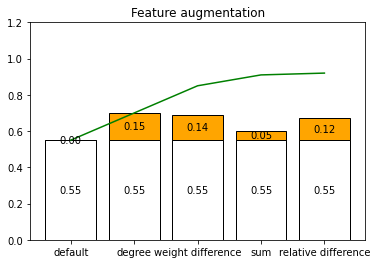
\includegraphics[scale=0.8]{figures/FeatureAugmentationLine}
    \caption{MNIST trained model. Average performance on 100 MNIST graphs}
    \label{Feature Augmentation Effect}
\end{figure}

The figure \ref{Feature Augmentation Effect} shows each feature's impact on performance. The default white column demonstrates the model's performance without any additional features. The green colored columns visualize the positive effect of adding a feature, while the last column represents the final result when all the features are added simultaneously. We can observe that every feature has a positive effect on the performance and gives the largest improvement so far compared to the other experiments.

With the features added to the nodes, we proceed to experiment with the aggregation functions for the message passing. In the table \ref{aggrtable} one can see how the performance changes depending on the aggregation function used.

\begin{table}[h!]
\centering
\begin{tabular}{|| c | c ||} 
 \hline
 Aggregation function & Performance compared to greedy \\ [0.5ex] 
 \hline\hline
 add & 92.0\% \\
 \hline
 sum & 89.5\% \\
 \hline
 mean & 90.2\% \\
 \hline
 min & 87.0\% \\
 \hline
 max & 94.4\% \\
 \hline
\end{tabular}
\caption{Aggregation function performance}
\label{aggrtable}
\end{table}

With fine-tuning of the models' hyperparameters and architecture, and augmenting node features having the most effect on the performance, results were moving closer to being reasonable. At this point, a full training set can be used to see more realistic results. The results were relatively promising, but further testing showed that, unfortunately, line graph transformation on large and dense enough graphs turned out to grow out of proportions and take too much time to process. Therefore, another architecture was considered.

\section{Edge prediction model}

Instead of converting edges into nodes, a model can give predictions on the edges directly. With this approach, there is less preprocessing needed and without line graph convertion the input does not grow in size, but the model now needs to have a layer for the edge prediction part of the model. The purpose of this layer is to classify the edges based on the embeddings produced by the initial model, this is described in more detail in the \hyperref[sec:architecture]{Architecture section}. A simple linear layer with $320$ neurons was chosen as a starting point for the edge prediction.

After training both the edge classification model and the line graph model on the 55000 MNIST graphs with the best hyperparameters discovered in previous section, the following results compared to the greedy algorithm were recorded: 101\% for edge classification and 103\% for line graph model.

The figure \ref{Model performance on MNIST} depicts how MNIST trained line graph and edge prediction model's compare in terms of performance on unseen MNIST graphs. The orange section of the bar represents the portion of the total weight that stemmed from the greedy algorithm solving the unsolved remains of the graphs.
\begin{figure}[H]
    \centering
    \hspace*{-2cm}
    \includegraphics[scale=1.0]{figures/LineVSEdgeOnMNIST}
    \caption{MNIST performance comparison}
    \label{Model performance on MNIST}
\end{figure}

Edge classification showed a slightly worse results on average than the line graph. In theory, this can be due to the line graph containing more structural information in it compared to the original one. Regardless of the slightly worse result, the edge classification approach was still favorable due to the large time consumption of the line graph conversion. Overall, the results themselves are rather promising. Both models manage to beat the greedy algorithm even when the greedy result is close to the optimal. However, running time was still a problem. Due to the small size of MNIST graphs, finding an optimal solution using the Blossom algorithm takes less time than using our \gls{gnn} model, because of the overhead computations needed for the neural network during the prediction phase, but the model should be able to catch up time-wise when given larger graphs. There is still the question of whether training on small graphs can help with larger graphs. The next step is to test the current model on a different graph - Cage10 from SuiteSparse. Cage10 is a graph with 11000 nodes and 100 000 edges. The results can be seen in figure \ref{model performance}:

\begin{figure}[H]
    \centering
    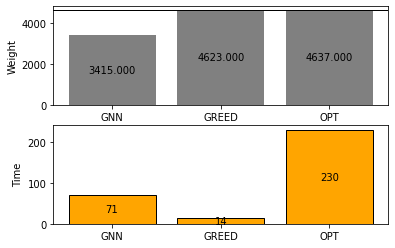
\includegraphics[scale=1.0]{figures/MNISTtrainCAGE10}
    \caption{MNIST trained model performance on cage10 graph}
    \label{model performance}
\end{figure}

As seen in figure \ref{model performance} the \gls{gnn} model manages to beat the optimal solver in terms of time, but it is noticeably worse in terms of total weight. Poor performance can be caused by the current training dataset. One of the main interests of the study was to see if the \gls{gnn} could be used on graphs larger than the ones it was trained on. It could be that the model fails to learn what is needed for larger graphs. Another reason could be that MNIST graphs have similar structures without enough variety to cover other graph types. One, of course, cannot include all the possible graphs in the training set, but the more data and variety the model gets during training the better. Therefore, another dataset was tested for training. A custom dataset consisting of randomly picked graphs from the SuiteSparse database. This custom dataset consists of 1000+ graphs with varying sizes and structures, between 100 and 10000 nodes.

Training the same model on the new dataset showed that the model struggled to learn the patterns. The flat information loss during training indicated that the model experienced difficulties learning the more diverse collection of graphs. Adding two more layers to the classifier module helped with the stagnating learning curve, but the number of epochs had to be increased up to 500, due to the learning curve slowing down significantly in comparison to the previous dataset. Further adding more layers or neurons did not give any noticeable difference in performance. Figure \ref{models performance comparison cage10} compares the performance of the new model trained using a custom dataset against the same model trained on MNIST graphs only. Figure \ref{custom data model performance cage10} shows the performance and the running time in seconds for \gls{gnn}, greedy and blossom's algorithms.

\begin{figure}[H]
    \centering
    \hspace*{-2cm}
    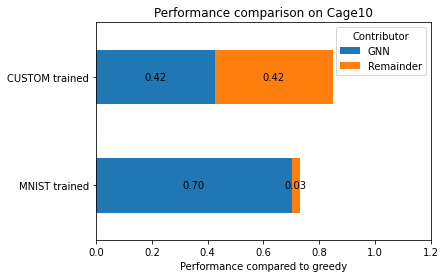
\includegraphics[scale=1.0]{figures/MNSITvsCUSTOMonCage10}
    \caption{MNIST vs CUSTOM dataset training model performance on cage10}
    \label{models performance comparison cage10}
\end{figure}

\begin{figure}[H]
    \centering
    \includegraphics[scale=1.0]{figures/CUSTOMtrainCAGE10}
    \caption{CUSTOM trained model performance on cage10 graph}
    \label{custom data model performance cage10}
\end{figure}

The custom-trained model does perform better than the MNIST-trained model on cage-10 graph. However, it is not necessarily the model's accuracy itself that is the reason for improvement. The edge prediction model seems to be rather indecisive on which nodes to match and half of the graph at the end is left unmatched, as opposed to the MNIST-trained model matching almost the whole graph. The large remainder is not necessarily a problem in itself, since one can use the model to only match the most important nodes with the highest probabilities and leave the rest to the greedy algorithm to achieve better results. However, the custom-trained model does not leave a large remainder in every case as figure \ref{models performance comparison mnist} demonstrates. 

\begin{figure}[H]
    \centering
    \hspace*{-2cm}
    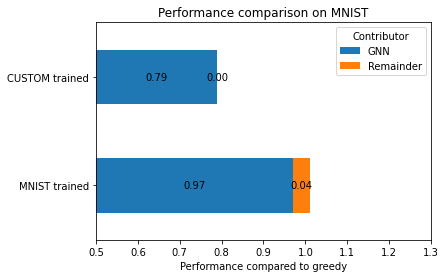
\includegraphics[scale=1.0]{figures/MNISTvsCUSTOMonMNIST}
    \caption{MNIST vs CUSTOM dataset training model performance on MNIST graphs}
    \label{models performance comparison mnist}
\end{figure}

Although the custom-trained model leaves no remainder for MNIST graphs, it performes noticeably worse than the model trained on exclusively MNIST graphs. The custom dataset had fewer but larger graphs than the ones in the MNIST dataset. Performance on MNIST graphs could be improved by adding a subset of MNIST graphs to the custom dataset, but that might not help with graphs from other datasets.

The current results indicate that our model might fit better for use on a narrow family of graphs that belong to a common dataset. Although, there are two more modifications that might improve the current model:

\begin{itemize}
\item Cases that leave large remainders lead to the idea of adjusting the matching threshold to focus the model on only searching for the most important edges. 
\item A common practice in algorithms is to add reduction rules to reduce the size of the graph without affecting the result, one can add a reduction preprocessing step to assist the model.
\end{itemize}

\subsection{Reduction}

Reduction rules in algorithms are used to cut down the graph's size by removing the parts that are either guaranteed to be in the solution or the opposite. In the case of \gls{mwm}, it is the edges that must be included in the solution regardless. Ideally, the neural network should be able to pick up such edges by itself, but it is still worth to test if there is any positive effect as well as to check if the model manages to grasp such rules by itself. The reduction rule itself is rather simple. If an edge that connects two nodes has larger weight than the sum of weights of the largest outgoing edges from each node, there is no reason not to pick it, since it is impossible to get a larger weight by matching these two nodes with other neighbours. Figure \ref{Reduction example} serves as an example, where it is clear that node one should be matched with node five, if not, one has to match both one and five to other nodes. Second-best matchings for both node one and five have $weight = 3$, giving a total weight of only six.

\begin{comment}
\begin{algorithmic}[H]
\KwData{$graph G$}
\ForAll{$edge e$}
	\If{$e.weight > weight sum of largest remaining edge weights of the nodes$}
		\STATE $Pick the edge$\;
	\EndIf
\EndFor
\end{algorithmic}
\end{comment}

\begin{figure}[H]
    \centering
    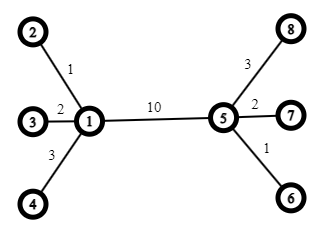
\includegraphics[scale=1.0]{figures/ReductionExample}
    \caption{Reduction example}
    \label{Reduction example}
\end{figure}

A couple of graphs from the custom dataset were used to test if the reduction helps and whether the model could identify reducible edges on its own. Some graphs had zero reducible edges, but in other cases such edges accounted for up to 5\% of the total number of edges. The model, however, did not seem to identify those edges in the graphs that contained them, and adding reduction as a preprocessing step did improve the results by between 2\% and 3\%. Since the reduction is based on the heaviest edges of the nodes, it is reasonable to add these node features to the model to potentialy help the model with finding the pattern for reduction. 

The new model was trained with two additional node features: largest edge weight and second-largest edge weight for each node. Adding such features could in theory have helped the model to find reducible nodes, but after training the new model with the new node features, the results did not improve. The reducible edges were still left unidentified by the model.

\subsection{Matching threshold}

Adjusting the threshold for picking the edges is another way to use the model. The model was initially set to consider all the edges that have a larger than 50\% chance of being in the solution. This matching threshold can be adjusted to, for example, only pick the edges with $90\%$ probability of being in the solution. This can help to focus the model on the edges that have a large impact on the total result, but might be otherwise ignored by a greedy algorithm. Additionally, it can be worth testing the removal of edges with low probabilities to see if the model can find edges that, if picked, inhibit the overall result.

\begin{figure}[H]
    \centering
    \hspace*{-1cm}
    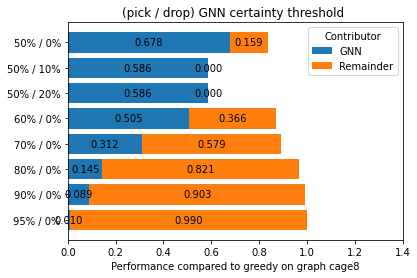
\includegraphics[scale=0.8]{figures/ThresholdDemo}
    \caption{Model threshold test on cage8 graph}
    \label{Model threshold test}
\end{figure}

Figure \ref{Model threshold test} shows how different thresholds affect the performance of the model. The x-axis labels represent the thresholds for picking and dropping the edge respectively. For example, in the second column labeled “$50\% / 10\%$”, $50\%$ refers to the lowest prediction certainty required for an edge to be in the solution and $10\%$ refers to the edges with prediction certainty of being in the solution lower than $10\%$ to be removed from the graph comepletely. The remainder is solved by the greedy algorithm.

The higher matching threshold does seem to improve the performance, but not enough to beat the greedy algorithm and most likely the increase is caused by the larger remainder being solved by th greedy algorithm due to fewer edges being above the threshold. Adding the drop threshold did not seem to work that well either. The model seems to assign very low scores to a lot of edges, which results in worse performance and no remainder for greedy algorithm to compensate. The reason for that is probably the weight class hyperparameter used during training, which makes the model prioritize less correctly finding nodes that should be ignored. The better approach could be to train the model specifically to find high value edges.

\section{Final results}

The final best model was tested on increasingly larger graphs from different sources. The final parameters of the model were:

\begin{enumerate}
\item Learning rate = $0.001$
\item Epochs = $500$
\item Mini-batch size = $1$
\item Node embedding network depth and width = $3$ layers, $640$ neurons each
\item Edge classifier network depth and width = $3$ layers, $320$ neurons each
\item Class weights = $0.1$ and $0.9$ for dropped and picked edges respectively
\item Weight decay = $0$
\item Match threshold = $70\%$
\item Added pre computed node features
	\begin{itemize}
	\item Degree - how many neighbours a node has.
	\item Sums of the weights. 	
	\item Weights sum relative to the neighbours.
	\item Weights sum difference compared to the neighbours.
	\end{itemize}
\item Agreggation function = Max
\end{enumerate}

\begin{figure}[H]
    \centering
    \hspace*{-2cm}
    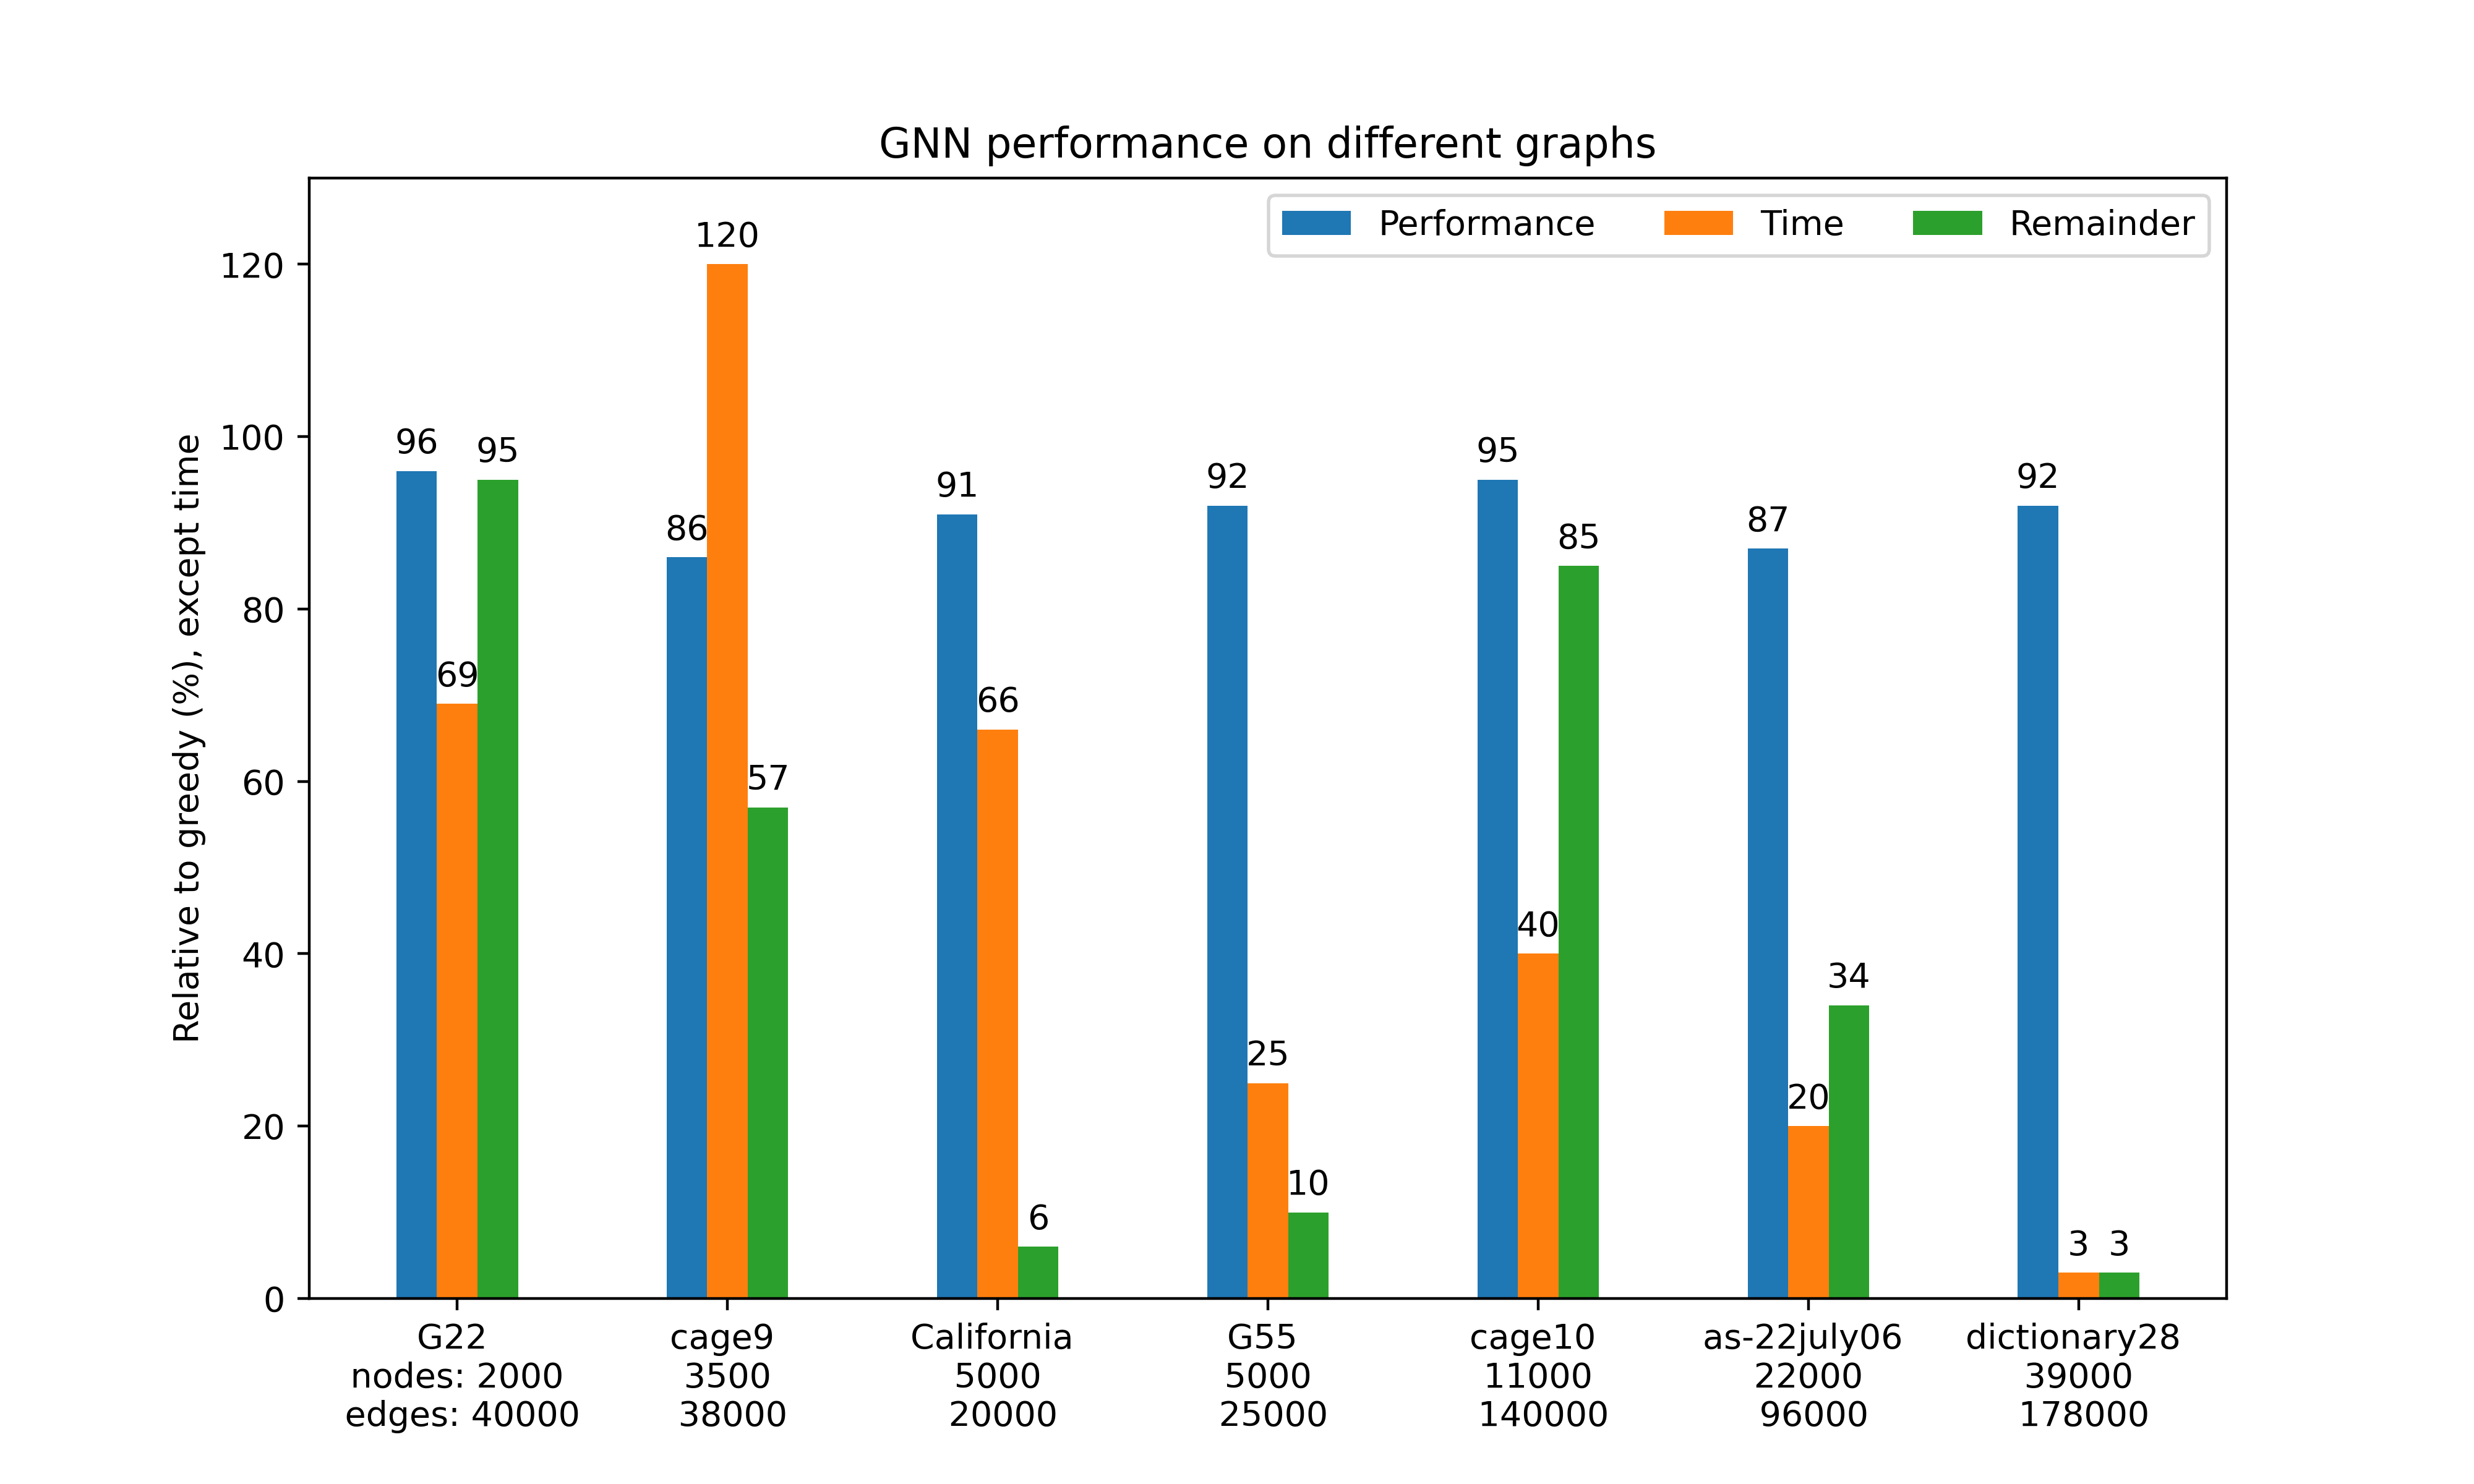
\includegraphics[scale=0.8]{figures/FINALResults}
    \caption{Final model performance}
    \label{Final model performance}
\end{figure}

Figure \ref{Final model performance} shows the performance of our final edge prediction model on the selection of increasingly larger graphs from different datasets. The blue colored columns stand for the models' performance on the graphs compared to the greedy algorithm. The green columns show the performance gained from solving the remainder of the graph with the greedy algorithm after the model could not find more edges. The orange column demonstrates the running time compared to the Blossom algorithm's running time.

Let's summarize the end results based on the main criteria.
\begin{itemize}
\item Performance: The total weight of the model's output seems to be rather stable at around 90\% of what a greedy algorithm produces, regardless of the size of the graph and the remainder. It seems to be rather challenging for the model to beat the greedy approach when, in most cases, it makes up at least 85\% of the total weight possible.
\item Running time: An exception in the sense that the time is shown in comparison to the time it takes to find the optimal solution. The reason for that is the fact that the model is always slower than the greedy algorithm. As expected, the benefit of using the \gls{gnn} can be seen as the size of the graphs increases. Smaller graphs take more time for the model to solve due to the overhead computations needed, but as the graphs grow the running time can get as small as 3\% of the Blossom algorithm.
\item Remainder: In some cases, the reason for the total weight being close to the greedy is the fact that the remainder makes up a large part of the graph, but it is not a consistent trend, and neither does it depend on the size of the graph. There are cases with equally good results where the remainder is below 10\% of the total graph. The fact that some graphs leave such a big remainder indicates that the training dataset is not good enough and the model is not trained well enough to handle such graphs.
\end{itemize}

\subsection{Weakness of the greedy algorithm}
\label{sec:greedybadcase}
On average, a greedy algorithm seems to show good results, but it is not hard to make a graph that abuses the greedy approach and results in poor performance.

\begin{figure}[H]
    \centering
    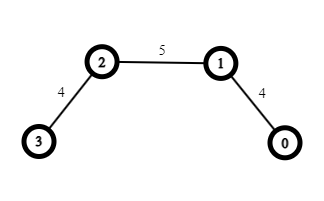
\includegraphics[scale=1.0]{figures/GoodCase}
    \caption{Good case for GNN}
    \label{Good case for GNN}
\end{figure}

Figure \ref{Good case for GNN} shows a simple case where the greedy algorithm results in total $weight = 5$. While our \gls{gnn} manages to get the optimal $weight = 8$. Graphs that we found on SuiteSparse and graphs with random weights result in the greedy algorithm achieving at least 85\% of the optimal result in the vast majority cases. Finding graphs that put greedy algorithm in disadvantage showed to be challenging, therefore, we modified the graphs used for testing using the principle showed in figure \ref{Good case for GNN}. 

\begin{figure}[H]
    \centering
    \hspace*{-4.5cm}
    \includegraphics[scale=0.7]{figures/MutatedGraphsTest.png}
    \caption{Greedy disadvantaged graphs}
    \label{Good case benchmark}
\end{figure}

Figure \ref{Good case benchmark} presents a performance comparison among the MNIST-trained model, custom-trained model, greedy algorithm, and Blossom algorithm when applied to graphs intentionally designed to challenge the greedy algorithm. For some of these modified graphs, our models outperform the greedy algorithm, a contrast to the results observed with the original graphs. However, for graphs from $cage$ and $G$ datasets, the performance is either worse than greedy or better than greedy, but significantly worse compared to the optimal solution. This suggests that our \gls{gnn} models may be more effective for certain types of graphs rather than universally applicable across all graph categories.

\chapter{Conclusion}


Results show that \gls{gnn}s are capable of solving \gls{mwm}, but the approaches presented in this work showed worse performance overall comapared to a simple standard greedy algorithm. The margin between the results was not big enough to indicate that the approach was completely sensless. Compared to the greedy algorithm model showed some level of "understanding" of the task at hand and in some special cases even manages to beat the greedy algortihm. It is worth mentioning that theese cases were manualy chosen because of the way they abuse the naiveness of the greedy algorithm, but it does still indicate that such cases do exist and therefore there is value in using \gls{gnn} instead of a greedy algorithm. 

\section{Future work}

The fact that \gls{gnn} in this work underperformed does not neccessary mean that the \gls{gnn}s are in general unfit for \gls{mwm} problem. There several potential improvements at hand. A deeper or wider model can be trained, meaning adding more layers as well as neurons to each layer to potentialy improve models ability to recognise complex patterns at the cost of longer training and prediction times. However for this particular architecture adding more layers showed little to no effect. Theres also a variety of different architectures that can be tested. A semi-supervised or an unsupervised approach is a good potential candidate where precomputing the optimal solution would not be needed. Instead the model can try to find the best solution by incentivising it to get as high weight sum as possible, resembeling a game in a way .

\section{Final words}

% Include more chapters as required.
%%=========================================

% Alternative 1 of printing glossaries & acronymes
%\renewcommand{\glossarypreamble}{\footnotesize}
%\printglossary[style=super, type=\glsdefaulttype] \let\cleardoublepage\clearpage
%\printglossary[style=super, type=\acronymtype]


%Alternative 2
%Simplified way of printing glossaries, slower than alt 1, but has better compatibility
\printnoidxglossaries

% Include more appendices as required.
%%=========================================
\clearpage
\DeclareRobustCommand{\VAN}[3]{#3}
\addcontentsline{toc}{chapter}{Bibliography}
\bibliographystyle{generators/myplainnat}
\bibliography{generators/refs}
\appendix
\titleformat{\chapter}[display]
  {\normalfont\large\bfseries}% <- font for label "Appendix A", default \huge
  {\chaptertitlename\ \thechapter}
  {20pt}
  {\large}% <- font for title, default \Huge

\chapter{Generated code from Protocol buffers}

\begin{lstlisting}[caption={Source code of something},label=Listing]
System.out.println("Hello Mars");
\end{lstlisting}
\end{document}
